%% Copernicus Publications Manuscript Preparation Template for LaTeX Submissions
%% ---------------------------------
%% This template should be used for copernicus.cls
%% The class file and some style files are bundled in the Copernicus Latex Package, which can be downloaded from the different journal webpages.
%% For further assistance please contact Copernicus Publications at: production@copernicus.org
%% https://publications.copernicus.org/for_authors/manuscript_preparation.html


%% Please use the following documentclass and journal abbreviations for discussion papers and final revised papers.

%% 2-column papers and discussion papers
\documentclass[journal abbreviation, manuscript]{copernicus}



%% Journal abbreviations (please use the same for discussion papers and final revised papers)


% Advances in Geosciences (adgeo)
% Advances in Radio Science (ars)
% Advances in Science and Research (asr)
% Advances in Statistical Climatology, Meteorology and Oceanography (ascmo)
% Annales Geophysicae (angeo)
% Archives Animal Breeding (aab)
% ASTRA Proceedings (ap)
% Atmospheric Chemistry and Physics (acp)
% Atmospheric Measurement Techniques (amt)
% Biogeosciences (bg)
% Climate of the Past (cp)
% Drinking Water Engineering and Science (dwes)
% Earth Surface Dynamics (esurf)
% Earth System Dynamics (esd)
% Earth System Science Data (essd)
% E&G Quaternary Science Journal (egqsj)
% Fossil Record (fr)
% Geographica Helvetica (gh)
% Geoscientific Instrumentation, Methods and Data Systems (gi)
% Geoscientific Model Development (gmd)
% History of Geo- and Space Sciences (hgss)
% Hydrology and Earth System Sciences (hess)
% Journal of Micropalaeontology (jm)
% Journal of Sensors and Sensor Systems (jsss)
% Mechanical Sciences (ms)
% Natural Hazards and Earth System Sciences (nhess)
% Nonlinear Processes in Geophysics (npg)
% Ocean Science (os)
% Primate Biology (pb)
% Proceedings of the International Association of Hydrological Sciences (piahs)
% Scientific Drilling (sd)
% SOIL (soil)
% Solid Earth (se)
% The Cryosphere (tc)
% Web Ecology (we)
% Wind Energy Science (wes)


%% \usepackage commands included in the copernicus.cls:
%\usepackage[german, english]{babel}
%\usepackage{tabularx}
%\usepackage{cancel}
%\usepackage{multirow}
%\usepackage{supertabular}
%\usepackage{algorithmic}
%\usepackage{algorithm}
%\usepackage{amsthm}
%\usepackage{float}
%\usepackage{subfig}
%\usepackage{rotating}


\begin{document}

\title{A neural network approach to estimate posterior distributions of Bayesian retrieval problems}


% \Author[affil]{given_name}{surname}

\Author[1]{Simon}{Pfreundschuh}
\Author[1]{Patrick}{Eriksson}
\Author[1]{David}{Duncan}
\Author[2]{Nina}{H{\aa}kansson}
\Author[2]{Anke}{Thoss}

\affil[1]{Department of Earth Space and Environment, Chalmers University of Technology, SE-41296 Gothenburg, Sweden}
\affil[2]{Swedish Meteorological and Hydrological Institute (SMHI), Norrköping, Sweden}
%% The [] brackets identify the author with the corresponding affiliation. 1, 2, 3, etc. should be inserted.



\runningtitle{TEXT}

\runningauthor{TEXT}

\correspondence{simon.pfreundschuh@chalmers.se}



\received{}
\pubdiscuss{} %% only important for two-stage journals
\revised{}
\accepted{}
\published{}

%% These dates will be inserted by Copernicus Publications during the typesetting process.


\firstpage{1}

\maketitle



\begin{abstract}
TEXT
\end{abstract}


\copyrightstatement{TEXT}


\introduction  %% \introduction[modified heading if necessary]

The retrieval of atmospheric quantities from remote sensing measurements
constitutes an inverse problem and generally does not admit a unique, exact
solution. Measurement and modeling errors as well as limited sensitivity of the
observation system forbid the assignment of a single, discrete solution to a
given observation. A meaningful retrieval should thus consist of a retrieved
value and an estimate of uncertainty describing a range of values that are
likely to produce a measurement similar to the one observed. However, even
if a retrieval method allows for explicit modeling of retrieval uncertainties,
their computation and representation is often possible only in an approximate
manner.

The Bayesian framework provides a formal way of handling the ill-posedness of
the retrieval problem and its associated uncertainties. In the Bayesian
formulation \citep{rodgers}, the solution of the inverse problem is given by the
a posteriori distribution $p(x | \vec{y})$, i.e. the conditional distribution of
the retrieval quantity $x$ given the observation $\vec{y}$. Under the modeling
assumptions, the posterior distribution represents all available knowledge about
the retrieval quantity $x$ after the measurement including all retrieval
uncertainties. Bayes' theorem states that the a posteriori distribution is
proportional to the product $p(\vec{y} | x)p(x)$ of the a priori distribution
$p(x)$ and the conditional probability of the observed measurement $p(\vec{y} |
x)$. The a priori distribution $p(x)$ represents knowledge that is available
about the quantity $x$ before the measurement and can be used to aid the
retrieval with supplementary information.

The a posteriori distribution of a retrieval can generally not be expressed in
closed form and different methods have been developed to compute the distribution
or approximations of it.

In cases that allow a sufficiently precise and efficient simulation of the
transmission of the measured radiation through the atmosphere, a forward model
can be used to guide the solution of the inverse problem. If such a forward
model is available, the most general method to compute the a posteriori
distribution are Markov chain Monte Carlo (MCMC) simulations. MCMC simulations
provide a way of iteratively generating samples from the a posteriori
distribution requiring only the specification of a priori knowledge and
measurement uncertainties in terms of easily computable probability
distributions. The disadvantage of MCMC simulations is that each retrieval
requires multiple evaluations of the forward model, which makes the method in
many cases computationally too demanding to be used in production.

A method that avoids potentially costly forward model evaluations during
the retrieval has been proposed by \cite{kummerow_1}. The method is based on
Monte Carlo integration of importance weighted samples in a retrieval database
$\{(\vec{y}_i, x_i)\}_{i = 0}^n$, which consists of pairs of observations $\vec{y}_i$
and corresponding values $x_i$ of the retrieval quantity $x$. The method will be
referred to in the following as Bayesian Monte Carlo integration (BMCI).
Eventhough the method is in general computationally less demanding than methods
involving forward model calculations during the retrieval, it may require the
traversal of a potentially large retrieval database. Furthermore, the
incorporation of ancillary data to aid the retrieval requires careful
stratification of the retrieval database, as it is performed in the GPROF
\citep{gprof} algorithm for the retrieval of rain profiles from GMI
measurements. Further applications of the method can be found for example in the
work by Rydberg (\citeyear{rydberg_2, rydberg_1}) or \cite{evans_2}.

The optimal estimation method \citep{rodgers}, in short OEM (also MAP, 1DVAR),
simplifies the Bayesian retrieval problem assuming that a priori knowledge and
measurement uncertainty can be described by Gaussian distributions and that the
forward model is only moderately non-linear. Under these assumptions, the a
posteriori distribution is approximately Gaussian and can be represented by its
mean value and covariance matrix. The retrieved values in this case are the mean
and maximum of the a posteriori distribution, which coincide for a Gaussian
distribution, as well as the covariance matrix describing the uncertainties in
the retrieval. In cases where an efficient forward model for the computation of
simulated measurements and corresponding Jacobians is available, the OEM has
become the quasi standard method for Bayesian retrievals. Nonetheless, even
neglecting the validity of the assumptions of Gaussianity and linearity, the
method is unsuitable for retrievals that involve complex radiative processes. An
example of such processes is the scattering of mircowave radiation by ice
clouds, which is generally too expensive to model online during the retrieval.

In contrast to the Bayesian retrieval methods discussed above, machine learning
provides a highly flexible approach to learn computationally efficient retrieval
mappings directly from data. Recent advances in machine learning have shown that
these methods are capable of learning complex relationships directly from
low-level data \citep{lecun}. Large amounts of training data from simulations,
collocated observations or in situ measurement as well as increasing amounts of
computational power available for training have made machine learning techniques
an interesting alternative to approaches based on (Bayesian) inverse modeling.
Numerous applications of deep learning regression methods to retrieval problems
can be found in recent literature \citep{holl, strandgren, hakansson}. All of
these examples, however, neglect the probabilistic character of the inverse
problem and provide only a scalar estimate of the retrieval. Uncertainty
estimates in these retrievals are provided in the form of expected errors
computed on independent test data, which is a clear drawback compared to
Bayesian methods.

In this article, quantile regression neural networks (QRNNs) are proposed as a
method to use deep neural networks to estimate the posterior distribution of
remote sensing retrievals. The aim of this approach is to combine the
flexibility and computational efficiency of machine learning methods with the
theoretrically sound handling of uncertainties in the Bayesian framework. 

After a formal description of QRNNs and the retrieval methods used to validate
the proposed approach in Section~\ref{sec:methods}, the implementation of the
methods in software is described in Section~\ref{sec:implementation}. In
Section~\ref{sec:synthetic}, a synthetic retrieval case is used to validate the
estimates of the posterior distribution against MCMC simulations and the BMCI
method. Finally, QRNNs are applied to a real world retrieval of cloud pressure
from MODIS observations in Section~\ref{sec:ctp}.

\section{Methods}
\label{sec:methods}

This section introduces the Bayesian retrieval formulation and the retrieval methods
used in the subsequent experiments. Two methods, Markov chain Monte Carlo simulations
and Baysesian Monte Carlo integration, for the computation of Bayesian a posteriori
distributions are presented. Furthermore, quantile regression neural networks are
presented as a machine learning based approach to estimate the a posteriori distribution
of Bayesian retrieval problems.

\subsection{The Retrieval Problem}

The problem under consideration is the retrieval of a scalar, physical quantity
$x \in \mathrm{R}$ from an indirect measurement given in the form of an observation
vector $\vec{y} \in \mathrm{R}^m$. In the Bayesian framework, the retrieval problem is
formulated as finding the posterior distribution $p(x | \vec{y})$ of the
quantity $x$ given the measurement $\vec{y}$. Formally, this solution can be
obatined by application of Bayes theorem:
\begin{equation}\label{eq:bayes}
  p(x | \vec{y}) = \frac{p(\vec{y} | x)p(x)}{\int p(x', \vec{y}) dx'}
\end{equation}
The a priori distribution $p(x)$ represents the knowledge about the quantity $x$ that
is available prior to the measurement. The a priori knowledge introduced into the
retrieval formulation acts as a regularizer on the ill-posed inverse problem and
ensures that the retrieval solution is physically meaningful.
If the retrieval quantity $x$ is a scalar, a convenient representation of the a
posteriori distribution is its cumulative distribution function
(CDF) $F_{x | \vec{y}}(x)$, which is defined as
\begin{equation*}
F_{x | \vec{y}}(x) = \int_{-\infty}^{\infty} p(x | \vec{y}) \: dx.
\end{equation*}

\subsection{Bayesian Retrieval Methods}

The a posteriori distribution in Equation (\ref{eq:bayes}) can generally not
be computed or sampled from directly. In the following two methods are presented
that are commonly used to compute the a posteriori distribution of Bayesian remote
sensing retrievals.

\subsubsection{Markov Chain Monte Carlo}

    Markov Chain Monte Carlo (MCMC) or Markov Chain simulation is a method
    to generate samples from arbitrary posterior distributions $p(x | \vec{y})$.
    It is based on drawing samples from an approximate distribution and
    refining these in a way such that the resulting sample distribution
    converges to the true distribution \citep{bda}.

    In this study, the Metropolis algorithm is used to implement MCMC. The
    Metropolis algorithm iteratively generates a sequence of states $\vec{x}_0,
    \vec{x}_1, \ldots$ based on a symmetric proposal distribution
    $J_t(\vec{x}^* | \vec{x}_{t-1})$. In each step of the algorithm, the
    distribution $J_t(\vec{x}^* | \vec{x}_{t-1})$ is used to generate a new
    proposal state $\vec{x}^*$ given the current state $\vec{x}_{t-1}$ of the simulation.
    The proposed state $\vec{x}^*$ is accepted ($\vec{x}_t = \vec{x}^*$) with
    probability $\text{min} \left \{1, \frac{p(\vec{x}^x |
      \vec{y})}{p(\vec{x}_{t-1} | \vec{y})} \right \}$. Otherwise it is rejected
    ($\vec{x}_t = \vec{x}_{t-1}$).

    If the proposal distribution is symmetric and satisfies the Markov chain property, the
    samples generated using the Metropolis algorithm are guaranteed to converge to the
    true a posteriori distribution. 

\subsubsection{Bayesian Monte Carlo Integration}

    The BMCI method is based on the use of importance sampling to approximate
    integrals over the a posteriori distribution of a given retrieval case. Consider an
    integral of the form
    \begin{equation}\label{eq:bmci_int}
     \int f(x') p(x'|\vec{y}) \: dx'.
    \end{equation}
    Applying Bayes' theorem, the integral can be written as
    \begin{equation*}
    \int f(x') \frac{p(x'|\mathbf{y}) p(x')}{p(\vec{y})} \: dx' &=
    \int f(x') \frac{p(\vec{y} | x')p(x')}
                    {\int p(\vec{y} | x'') \: dx''} \: dx'.
    \end{equation*}
    The last integral can be approximated by a sum over an observation
    database $\{(\vec{y}_i, x_i)\}_{i = 1}^n$ that is distributed according
    to the a priori distribution $p(x)$:
    \begin{equation*}
    \int f(x') p(x' | \vec{y}) \: dx' & = \frac{1}{C}  \sum_{i = 1}^n w_i(\mathbf{y}) f(x_i)
            .
    \end{equation*}
    The weights $w_i(\vec{y})$ are proportional to the probability
    of the observed measurement $\vec{y}$ conditional on the database
    measurement $\vec{y_i}$, which is usually assumed to be multivariate
    Gaussian with covariance matrix $\vec{S}_o$:
    \begin{equation*}
    w_i(\vec{y}) = \frac{1}{C} \exp \left \{- \frac{(\vec{y} - \vec{y}_i)^T \vec{S}_o^{-1}
                                       (\vec{y} - \vec{y}_i)}{2} \right \}
    \end{equation*}
    The normalization factor $C$ is given by $C = \sum_{i = 1}^n w_i(\vec{y}).$ By
    approximating integrals of the form (\ref{eq:bmci_int}), it is possible to
    estimate expectation value and variance of the posterior distribution by choosing $f(x) =
    x$ and $f(x) = (x - \mathcal{E}(x | \vec{y}))^2$, respectively. Likewise it
    is possible to approximate the cumulative density function of the posterior
    using
    \begin{equation}
    \label{eq:cdf}
    F_{x | \vec{y}}(x) &= \int_{-\infty}^x  p(x') \: dx'\approx \sum_{x_i < x}^n w_i(\mathbf{y}).
    \end{equation}

\subsection{Machine Learning}

In the field of machine learning, regression problems are typically approached
by training a parametrized model $f: \vec{x} \mapsto \vec{y}$ to predict a
desired output $\vec{y}$ from given input $\vec{x}$.

Unfortunately, the use of the variables $\vec{x}$ and $\vec{y}$ in
machine learning is directly opposite to their use in inverse theory. However,
for the remainder of this section the variables $\vec{x}$ and $\vec{y}$ will be
used to denote, respectively, the input and output to the machine learning model
in order to be consistent with the common notation in the field of machine
learning. The reader must just keep in mind that the method is applied in the
later sections to predict a retrieval quantity $x$ from a measurement $\vec{y}$.

\subsubsection{Supervised Learning and Loss Functions}

A common way of training machine learning methods is supervised training, in which
the machine learning model $f$ is trained on a training set
$\{\vec{x}_i, \vec{y}_i\}_{i = 1}^n$ consisting of input values $\vec{x}_i$ and
corresponding expected output values $\vec{y}_i$. The training is performed by
finding model parameters that minimize the mean of a given loss function
$\mathcal{L}(f(\vec{x}), \vec{y})$ on the training set.

The arguably most common loss function for regression tasks is the
squared error loss 
\begin{equation}
  \mathcal{L}_{se}(f(\vec{x}), \vec{y}) &= (f(\vec{x}) - \vec{y})^T (f(\vec{x}) - \vec{y}),
\end{equation}
which trains the model $f$ to minimize the mean squared distance
of the neural network prediction $f(\vec{x})$ from the expected output
$\vec{y}$.
If the estimand $\vec{y}$ is a random vector drawn from a conditional
probability distribution $p(\vec{y} | \vec{x})$, a regressor trained using a
sqared error loss function learns to predict the conditional expectation value of
the distribution $p(\vec{y} | \vec{x})$ \citep{bishop_mdn}. Depending on the
choice of the loss function, it is also possible to learn other statistics of
the distribution $p(\vec{y} | \vec{x})$ from the training data.

\subsubsection{Quantile Regression}

    Given the cumulative density function $F(x)$ of a probability distribution
    $p$, its $\tau\text{th}$ quantile $x_\tau$ is defined as
    \begin{align}
    x_\tau &= \inf \{x \: : \: F(x) \geq \tau \},
    \end{align}
    i.e. the greatest lower bound of all values of $x$ for which $F(x) \geq \tau$.
    As it has been shown by \citet{koenker}, the $\tau\text{th}$ quantile $x_\tau$ of $F$
    minimizes the expectation value $\mathcal{E}_x\left ( \mathcal{L}_\tau(x_\tau, x) \right) = \int_{-\infty}^\infty \mathcal{L}_\tau(x_\tau, x') p(x') \: dx'$
    of the function
    \begin{align}\label{eq:quantile_loss}
      \mathcal{L}_{\tau}(x_\tau, x) &=
      \begin{cases}
        \tau |x - x_\tau|, & x_\tau < x \\
        (1 - \tau)|x - x_\tau|, &\text{otherwise}
        \end{cases}
    \end{align}

    By training a machine learning regressor $f$ to minimize the quantile loss
    function $\mathcal{L}_\tau(f(\vec{x}), y)$ over a training set $\{\vec{x}_i,
    y_i\}_{i = 1}^n$, the regressor learns to predict the quantiles of the
    conditional distribution $p(y | \vec{x})$. This can be extended to obtain an
    approximation of the cumulative distribution function of $F_{y | \vec{x}}(y)$ by
    training the network to estimate multiple quantiles of $p(y | \vec{x})$.

\subsubsection{Neural Networks}

A neural networks is a computing model that computes a vector of output
activations $\vec{y}$ from a vector of input activations $\vec{x}$. Feed-forward
artificial neural networks (ANNs) compute the
vector $\vec{y}$ by application of a given number of subsequent, learnable
transformations to the input activations $\vec{x}$:
\begin{align*}
    \vec{x}_0 &= \vec{x}\\
    \vec{x}_i &= f_{i}
    \left ( \vec{W}_{i} \vec{x}_{i - 1}+ \vec{\theta}_i \right ) \\
    \hat{\vec{y}} &= \vec{x}_{n}
\end{align*}
The activation functions $f_i$ as well as the number and sizes of the
hidden layers $\vec{x}_1, \ldots, \vec{x}_{n-1}$ are fixed, structural parameters of a neural
network model. The learnable parameters of the model are the weight
matrices $\vec{W}_i$ and bias vectors $\vec{\theta}_i$ of each layer.

Neural networks can be efficiently trained in a supervised manner by using
gradient based minimization methods to find suitable weights $\vec{W}_i$ and
bias vectors $\vec{\theta}_i$. Hence, all that is required to use a neural networks
for quantile regression is the use of the mean quantile loss function
$\mathcal{L}_\tau$ as minimzation criterion during the training of network.
    
\subsection{Evaluating Probabilistic Predictions}

  A problem that remains is how to compare two estimated posterior distributions
  $p'(x | \vec{y}), p''(x | \vec{y})$ against a single sample $x$ from the true
  a posteriori distribution $p(x | \vec{y})$. A probabilistic prediction of an
  observed value $x$ should be sharp, i.e. concentrated in the vicinity of
  $x$, but at the same time well calibrated, i.e. predicting probabilities
  that truthfully reflect observed frequencies \citep{gneiting_2}. Such summary
  measures for the evaluation of predicted conditional distributions are called
  scoring rules \citep{gneiting}. An important property of scoring rules
  is propriety, which formalizes the concept of the scoring rule rewarding both
  sharpness and calibration of the prediction. Besides providing reliable
  measures for the comparison of probabilistic predictions, proper scoring rules
  can also be used as loss function in supervised learning to incentivize
  statistically consistent predictions.

  As noted by \cite{gneiting}, the quantile loss function given in equation
  (\ref{eq:quantile_loss}) is a proper scoring rule for quantile estimation
  and can thus  be used to compare the skill of different methods for
  quantile estimation.

  Another proper scoring rule for the evaluation of estimations of a
  cumulative distribution function $F$ is the continuous ranked probability
  score (CRPS):
  \begin{align}\label{eq:crps}
    \text{CRPS}(F, x) &= \int_{-\infty}^{\infty} 
    \left ( F(y) - I_{x \geq y} \right )^2 \: dy
  \end{align}
  For the methods used in this article the integral  can only
  be evaluated approximately. The exact way in which this is done for each
  method is described in detail in Section \ref{sec:implementation}.

  The scoring rules presented above evaluate probabilistic predictions against a
  single observed value. However, since MCMC simulations can be used to generate
  samples from the true a posteriori distribution, the probabilistic predictions
  obtained from BMCI and QRNN can also be compared directly to the a posteriori
  distributions obtained using MCMC. In the idealized case of the modeling
  assumptions underlying the MCMC simulations being true, the sampling
  distribution obtained from MCMC will converge to the true posterior and can
  therefore be used as a ground truth to assess the predictions obtained using
  the QRNN and BMCI methods.

\section{Implementation}
\label{sec:implementation}

  In this section the implementation of the retrieval methods used in the
  subsequent experiments is described. All three methods (MCMC, BCMI, QRNN) have
  been implemented in Python \citep{python} and released as parts of the typhon
  \citep{typhon} software package. The code for all calculations presented in
  this paper is made available in the form of jupyter notebooks through public
  repositories \citep{predictive_uncertainty, smhi}.

\subsection{Markov Chain Monte Carlo}

   The MCMC retrieval presented in Section~\ref{sec:synthetic} are based on
   a Python implementation of the Metropolis algorithm \citep[Ch. 12]{bda}.
   The implementation is designed to use the ARTS amtospheric radiative
   transfer simulator \citep{arts_1, arts_2} as forwad model and has been
   integrated into the typhon package.

   The MCMC retrieval computes the a posteriori distribution of the integrated
   column water vapor from passive microwave observations. The state space in
   which the retrieval is performed is given by the temperature and water vapor
   profiles of a plane parallel atmsophere. Proposal states are generated from a
   random walk using the a priori covariance matrix scaled by an adaptive factor
   that aims to keep the acceptance rate close to the optimal $21\%$
   \citep{bda}.

   A single MCMC retrieval consists of 8 independent runs, that are started with
   different random states sampled from the a priori distribution. Each run
   starts with a warm-up phase followed by an adaptive phase during which the
   scaling of the covariance matrix of the proposal distribution is adapted. This is
   followed by a production phase during which 5000 samples of the a posteriori
   distribution are generated. Of these 5000 only 250 are kept in order to decrease
   the correlation between the samples. To ensure sufficient convergence of the
   simulations, the scale reduction factor $\hat{R}$ and the effective number of
   independent samples \citep[eqs. (11.12), (11.13)]{bda} are computed. The
   retrieval is discarded if the values are not smaller than 1.1 and larger than
   100, respectively.
   
\subsection{Bayesian Monte Carlo Integration}

  Also the BMCI method has been implemented in python and integrated into the
  typhon package. The implementation provides functionality to speed up
  calculations by excluding entries that are guaranteed to have a smaller weight
  than a given limit. For the experiments presented below this was not used
  since computational performance was not considered critical. In addition to
  retrieving the first two moments of the posterior distribution, the
  implementation also provides functionality to retrieve the posterior CDF using
  Equation (\ref{eq:cdf}). Approximate posterior quantiles are computed by
  interpolating the inverse CDF at the desired quantile values. To compute the
  CRPS score for a given retrieval, the trapezoidal rule is used to perform the
  integral over the values $x_i$ in the retrieval database $\{\vec{y}_i,
  x_i\}_{i = 1}^n$.

\subsection{Quantile Regression Neural Networks}

    The implementation of quantile regression neural networks that has been
    developed is based on the Keras Python package for deep learning
    \citep{keras}. In order to enable the training of neural networks to predict
    quantiles, the quantile loss function $\mathcal{L}_\tau(x_\tau, x)$ has been
    implemented as a Keras-compatible loss function. The function can be
    initiated with a sequence of quantile fratctions $\tau_1, \ldots, \tau_k$
    allowing the neural network to learn to predict the corresponding quantiles
    $x_{\tau_1}, \ldots, x_{\tau_k}$.

    In addition to that, customized data generators have been added to the
    implementation in order to allow the incorporation of information on
    measurement uncertainty into the training process. If the training data is
    noise free, the data generator can be used to add Gaussian noise to each
    training batch according to the assumptions on measurement uncertainty. The
    noise is added only directly before the data is passed to the neural network
    keeping the original training data noise free. This ensures that the network
    does not see the same, noisy training sample twice during training.

    The QRNN implementation also provides support for adversarial training.
    While the general motivation for adversarial training is making neural
    network predictions more robust \citep{goodfellow_2}, its effect is similar
    to the augmentation of training data through the addition of noise to the
    input data. It has been proposed as a method to improve the calibration of
    probabilistic predictions from neural networks by \cite{lakshminarayanan}.

    The fast gradient sign method proposed by \citet{goodfellow_2} is used
    to implement adversarial training. Each training batch $(\vec{y}_i, \vec{x}_i)$
    consisting of $m$ input samples $\vec{y}_i \in \mathrm{R}^{m \times n}$ and
    expected outcomes $\vec{x}_i \in \mathrm{R}^m$ is augmented with a perturbed
    batch $(\vec{\tilde{y}}_i, \vec{x}_i)$ where $\vec{\tilde{y}}_i \in
    \mathrm{R}^{m \times n}$ is such that
    \begin{align}
      \vec{\tilde{y}}_i = \vec{y}_i + \delta_\text{adv} \text{sign} \left (
      \frac{d \mathcal{L}_\tau(\hat{\vec{x}}_\tau(\vec{y}_i), x)}{d\vec{y}_i} \right
      )
    \end{align}

    Here $\hat{\vec{x}}_\tau(\vec{y}_i)$ is the output predicted by the neural
    network for the input $\vec{x}_i$. The batch presented to the network is
    then simply given by the concatenation of the two batches.

   For the training of the neural network an adaptive form of stochastic batch
   gradient descent is used. During training, loss is monitored on a validation
   set. When the loss on the validation set hasn't decreased for a certain number
   of epochs, the training rate is reduced by a given reduction factor. The
   training is stopped when a predefined minimum learning rate is reached.

   The reconstruction of the CDF from the estimated quantiles is obtained
   by using the quantiles as nodes of a piece-wise linear approximation and
   extending the first and last segements out to 0 and 1, respectively.
   This approximation is also used to compute the CRPS score on the test
   data.



\section{Application to a Synthetic Retrieval Case}
\label{sec:synthetic}

  In this section the synthetic retrieval that is used to evaluate the
  performance of the BMCI and QRNN methods against MCMC is presented. The
  influence of different hyperparameters on the performance of the QRNN is
  investigated and finally the performance of the two methods is compared with
  respect to the size of the training database.

\subsection{Retrieval Setup}

   For this experiment, the retrieval of column water vapor (CWV) from passive
   microwave observations over the ocean is considered. The state of the
   atmosphere is represented by profiles of temperature and water vapor
   concentrations on 15 pressure levels between $10^3$ and $10^1\unit{hPa}$. The
   variablility of these quantities has been estimated based on ECMWF ERA
   Interim data \citep{era_interim} from the year 2016 restricted to latitudes
   between $23^\circ$ and $66^\circ$ North. Parametrizations of the multivariate
   distributions of temperature and water vapor were obtained by fitting a joint
   multivariate normal distribution to the temperature and the logarithm of
   water vapor concentrations. The fitted distribution represents the a priori
   knowledge on which the simulations are based.

\subsection{Radiative Transfer Simulations}

   The Atmospheric Radiative Transfer Simulator (ARTS) \citep{arts} is used to
   simulate satellite observations of the atmsopheric states sampled from the a
   priori distribution. The observations consist of simulated brightness
   temperatures from five channels at $23, 88, 165, 183 \unit{GHz}$
   (c.f. Table \ref{tab:channels}) of the ATMS sensor.

\begin{table}[hbpt]
\centering
\begin{tabular}{|r|c|c|}
    \hline
    Channel & Center Frequency           & Bandwidth                \\ 
    \hline
                  1 & $23.8 \unit{GHz}$ & $270 \unit{GHz}$ \\
                  2 & $88.2 \unit{GHz}$ & $500 \unit{GHz}$ \\
                  3 & $165.5\unit{GHz}$ & $300 \unit{GHz}$ \\
                  4 & $183.3\unit{GHz}$ & $3000\unit{GHz}$ \\
                  5 & $183.3\unit{GHz}$ & $1000\unit{GHz}$ \\
    \hline
\end{tabular}
\caption{Observation channels used for the synthetic retrieval of column water vapor}
\label{tab:channels}
\end{table}

   The simulations take into acount only absorption and emission from water
   vapor. Ocean surface emissivities are computed using the FASTEM \cite{fastem}
   model without taking into account surface winds. The sea surface temperature
   is assumed to be equal to the temeperature at the highest pressure level but
   no lower than $270\unit{K}$. Sensor characteristics and absorption
   lines are taken from the ATMS sensor descriptions that are provided within
   the ARTS XML Data package. Simulations are performed assuming a
   plane-parallel atmsophere and neglecting polarization.

\subsection{QRNN Model Selection}

 The structure of a QRNN model that is used for the retrieval is specified by the
 following hyperparamters: (1) the number of hidden layers, (2) the width of
 the hidden layers, (3) the activation functions of each layer. In addition to
 that, the following parameters define the training process: (4) the batch size
 used for stochastic gradient descent, (5) the minimum learning rate at which
 the training is stopped, (6) the learning rate decay factor, and (7) the
 number of epochs without decrease of loss on the validation set before
 the learning rate is reduced.

  To investigate the influence of these parameters on the performance of the
  QRNN, 10-fold cross validation has been used to estimate the performance
  impact of different hyperparameter configurations. Since the complete
  hyperparamter space is too large to be explored exhaustively, grid search was
  performed to find the approximately optimal structural hyperparameters (1),
  (2), (3). This was followed by a grid search over the training parameters
  (4), (5), (6) and (7) for the best performing configuration found in the
  first search.

  The full results for the grid search for optimal structural parameters are
  given in Table \ref{tab:model_selection} in the Appendix. The results show a
  large difference between using linear activations as opposed to non-linear
  activations. This is expected since a linear network can only model linear
  relations between the input variables. While the performance of the networks
  with non-linear activations is comparable, the results indicate a performance
  advantage for networks with ReLU activation functions. Performance is
  significantly increased when increasing the number of hidden layers from one
  to two as well as the width from 16 up to 64 neurons. For both these
  parameters performance saturates if the they are increased further. Based on
  these results, a network with three hidden layers and 128 neurons each has
  been chosen for the comparison against BMCI.

  The optimization of the training parameters showed that best performance is
  obtained for slow training with a small learning rate reduction factor of
  $1.5$ and decreasing the learning rate only after $10$ training epochs
  without reduction of the validation loss. No significant increase in
  performance could be observed for values of the learning rate minimum below
  $10^{-4}$. With respect to the batch size, the best results were obtained for
  a batch size of 128 samples.

\subsection{Comparison Against MCMC}

  The synthetic retrieval has been set up so that MCMC simulations can be used
  to compute atmospheric states whose distribution converges to the true a
  posteriori distribution. This allows the comparison of the predicted a
  posteriori distributions obtained from QRNN and BMCI against the a posteriori
  distribution obtained from MCMC simulations.

  In addition to a single QRNN also the performance of an ensemble of QRNNs is
  be investigated. The tests in this subsection are performed with a single QRNN
  as well as with an ensemble consisting of 10 QRNNs. The predictions from the
  ensemble are obtained by averaging the predictions from each network in the
  ensemble.

  To provide a rough, visual impression of the performance of BMCI and the QRNNs
  compared to MCMC, the results of 6 retrieval cases are displayed in
  Figure~\ref{fig:cdfs}. The choice of the retrieval cases is based on the
  Kolmogorov-Smirnov (KS) statistic, which corresponds to the maximum absolute
  deviation of the predicted CDF from the baseline obtained by MCMC
  simulation. The first row displays the cases corresponding to the 1st, 50th
  and 99th percentile of the distribution of KS values of predictions obtained
  using BMCI. The second row displays the corresponding cases for the QRNN
  method.

  In the displayed cases, both methods are generally successful in estimating the
  MCMC posterior. Only for the $99$th percentile of the BMCI KS value distribution,
  the BMCI prediction shows siginificant deviations from the baseline. The jumps
  in the estimated a posteriori CDF  indicate that the deviations are due to
  undersampling of the input space in the retrieval database. This results in 
  overproportionally high weights attributed to the few entries close to the
  observation. It is interesting to note, that for this specific case the QRNN
  provides a better estimate of the a posteriori CDF even though both
  predictions are based on the same retrieval database.

  \begin{figure}[hbpt!]
    \centering
    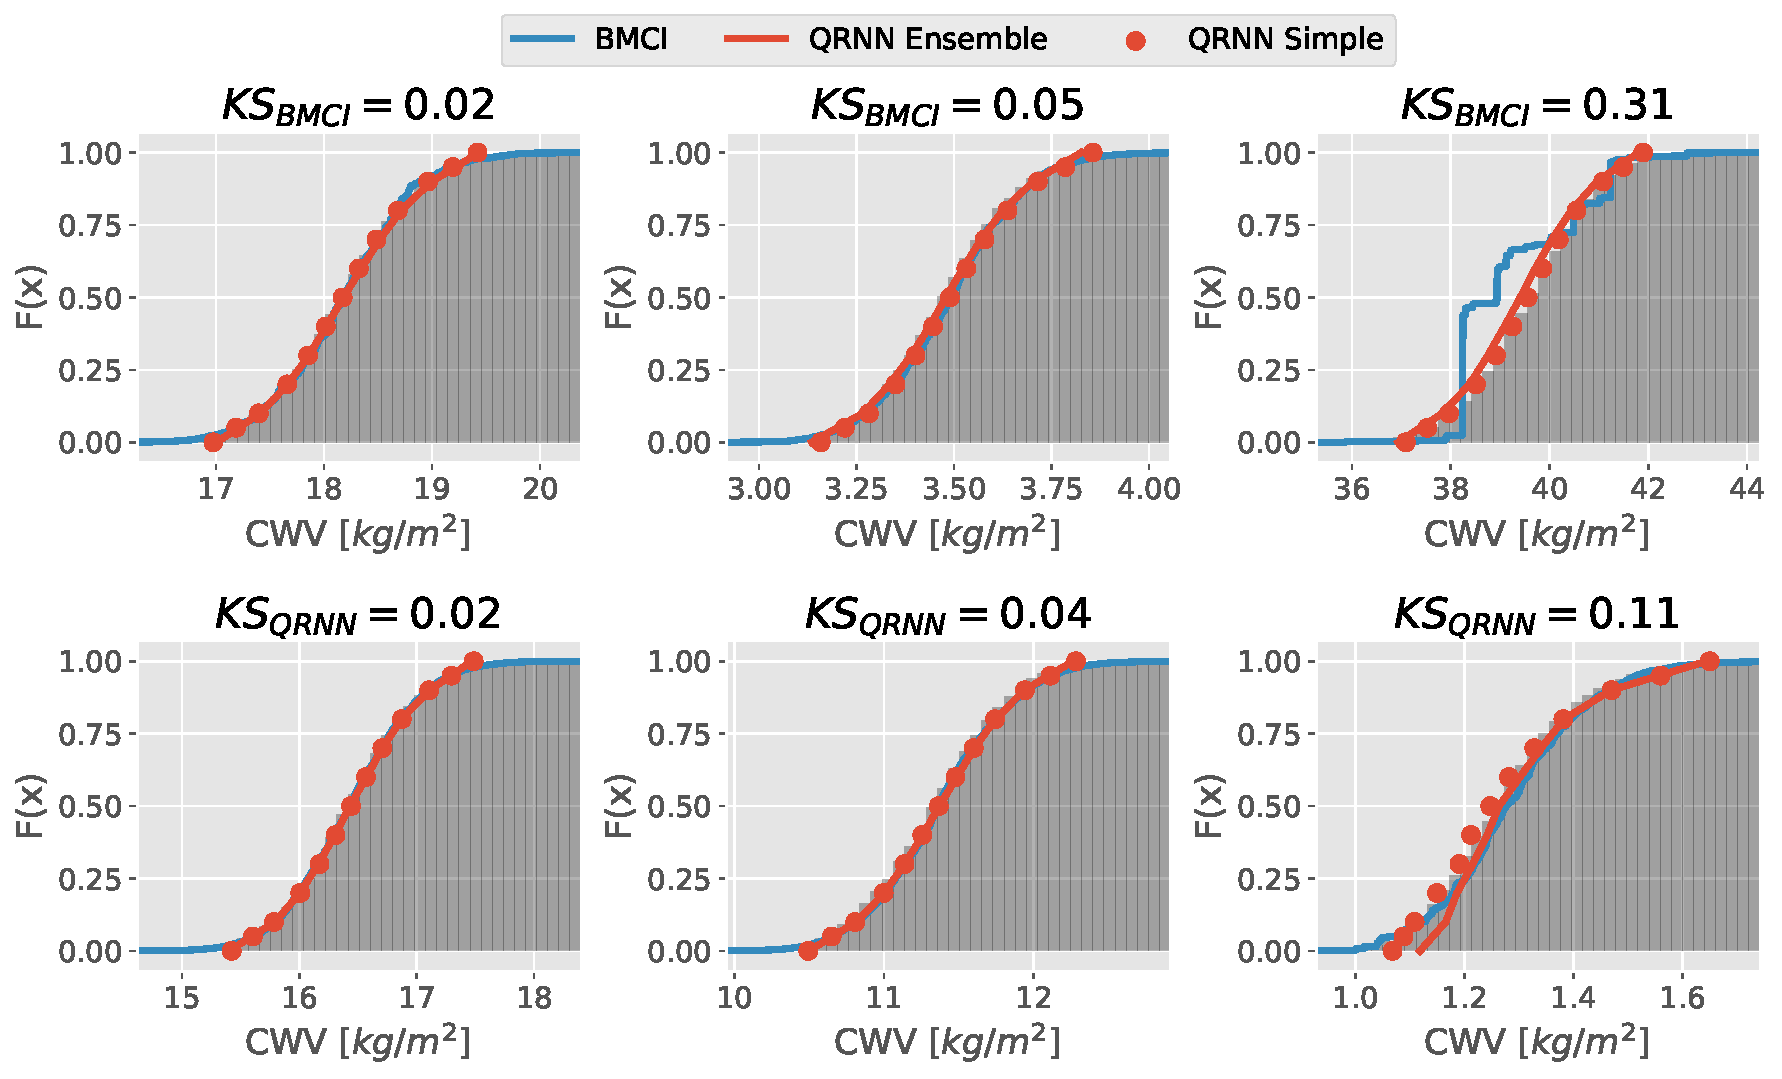
\includegraphics[width = 0.8\linewidth]{../plots/posterior_cdfs}
    \caption{Retrieved a posteriori CDFs a predicted by MCMC (grey), BMCI (blue),
      a single QRNN (red line) and an ensemble QRNN (red marker). Cases displayed in the first
      row are the 1st, 50th, 99th percentiles of the distribution of the Kolmogorov-Smirnov
      statistic of BMCI compared to the MCMC baseline. The second row displays the
      same percentiles of the distribution of the Kolmogorov-Smirnov statistic of the
      single QRNN predictions compared to MCMC.}
    \label{fig:cdfs}
  \end{figure}

  To obtain a more comprehensive view on the performance of QRNNs and BMCI, the
  predictions obtained from both methods are compared to those obtained from
  MCMC for a total number of 6500 test cases. For the comparison, define the
  effective quantile fraction $\tau_{\text{eff}}$ as the fraction of MCMC
  samples that are less than or equal to the estimated quantile $x_\tau$
  obtained from QRNN or BMCI. That is, the value $\tau_\text{eff}$ corresponds
  to the actual quantile fraction that the predicted $\tau$th quantile
  corresponds to with respect to the a posteriori distribution obtained from
  MCMC. The resulting distributions of the effective quantile fractions for BMCI
  and QRNNs are displayed in Figure~\ref{fig:quantile_fractions} for the
  estimated quantiles for $\tau = 0.1, 0.2, \ldots, 0.9$.

  \begin{figure}[hbpt!]
    \centering
    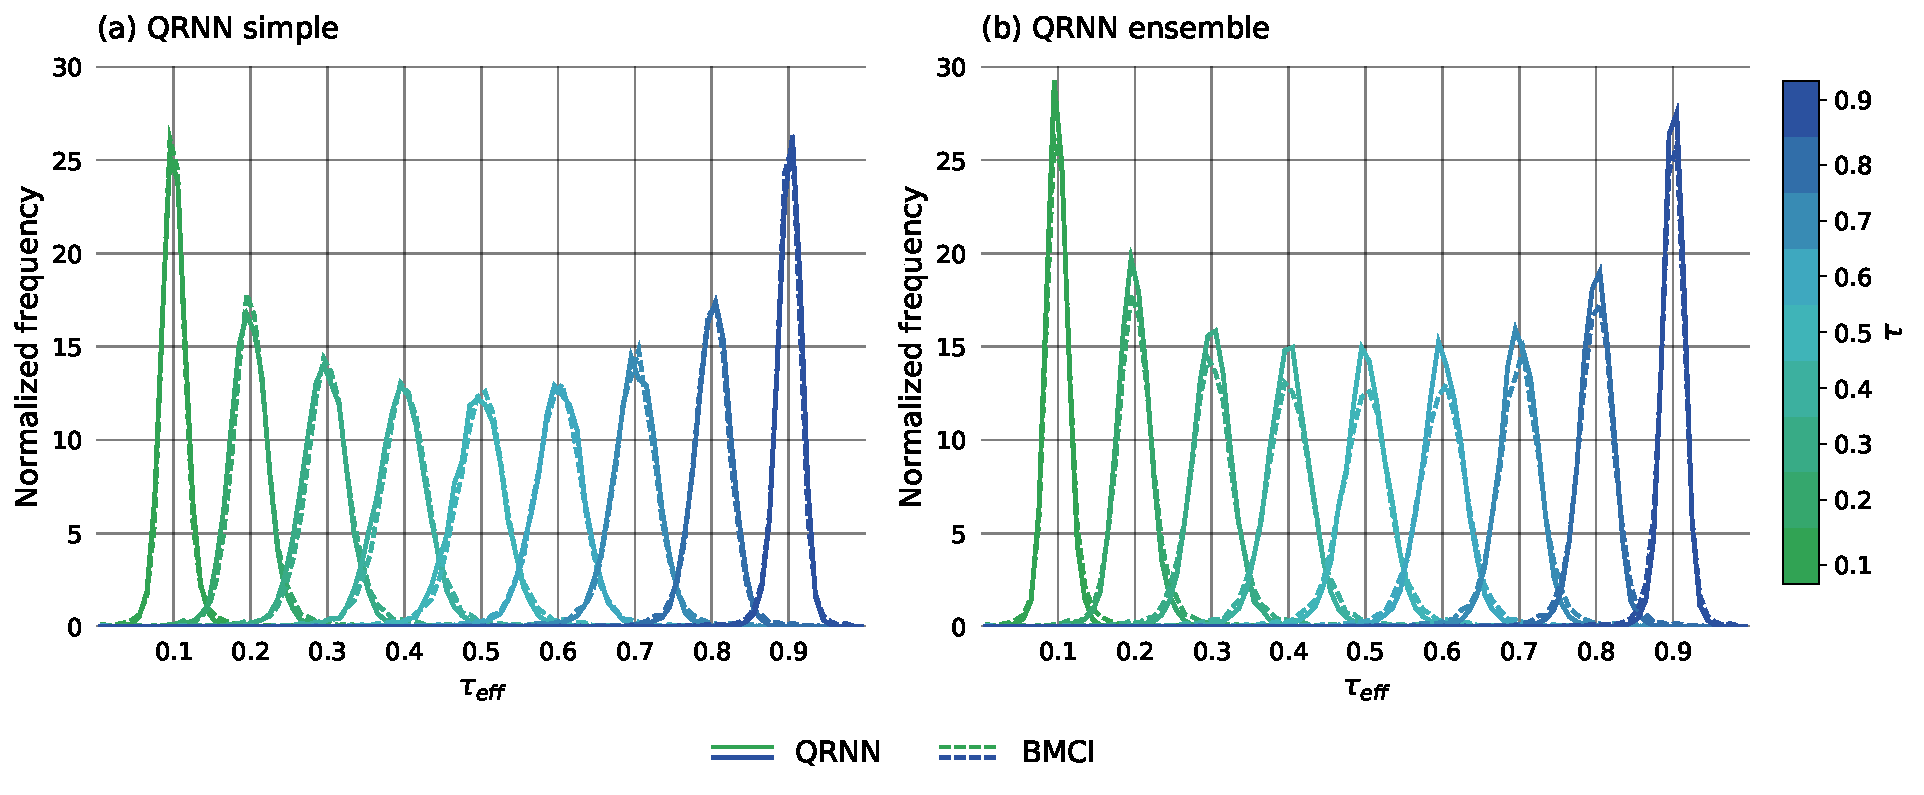
\includegraphics[width = 0.8\linewidth]{../plots/quantile_fractions}
    \caption{Distribution of effective quantile fractions $\tau_\text{eff}$ achieved by
      QRNN and BMCI on the test data. The left-hand plot displays the performance of a
      single QRNN compared to BMCI, the right-hand plot the performance of the ensemble.}
    \label{fig:quantile_fractions}
  \end{figure}

  For an ideal estimator of the quantile $x_\tau$, the resulting distribution
  would be a delta function centered at $\tau$. The results show that both, BMCI
  and QRNN, provide unbiased estimates of the quantiles of the a posterior
  distribution. Furhermore, both methods achieve equal precision in predicting
  the a posteriori quantiles.

\subsection{Training Set Size Impact}

Finally, it is investigated how the size of the training data used in the
training of the QRNN or as retrieval database for BMCI affects the performance
of the retrieval. This has been done by randomly generating training subsets
from the original training set with sizes logarithmically spaced between $10^3$
and $10^6$ samples. The data used to compare QRNNs and BMCI is a separate test
set consisting of observations and corresponding true CWV values. For each size,
five random training subsets have been generated and used to retrieve the test
data with QRNNs and BMCI.

Figure~\ref{fig:mape_crps} displays the means of the mean absolute percentage
error (MAPE, left panel) and the CRPS (right panel) achieved by both methods on
the differently sized training sets. The shaded background displays the range of
two standard deviations around the mean of the observed. The MAPE is computed by
comparing the predicted medians of the posterior distribution obtained from BMCI
and QRNN against the true CWV that was used in the simulation.

As expected, the performance of both methods improves with the size of the
training set. With respect to the MAPE, both methods perform equally well for a
training set size of $10^6$, but the QRNN outperforms BMCI for all smaller
training set sizes. With respect to CRPS, the QRNN has a slight advantage
over BMCI.

  \begin{figure}[hbpt!]
    \centering
    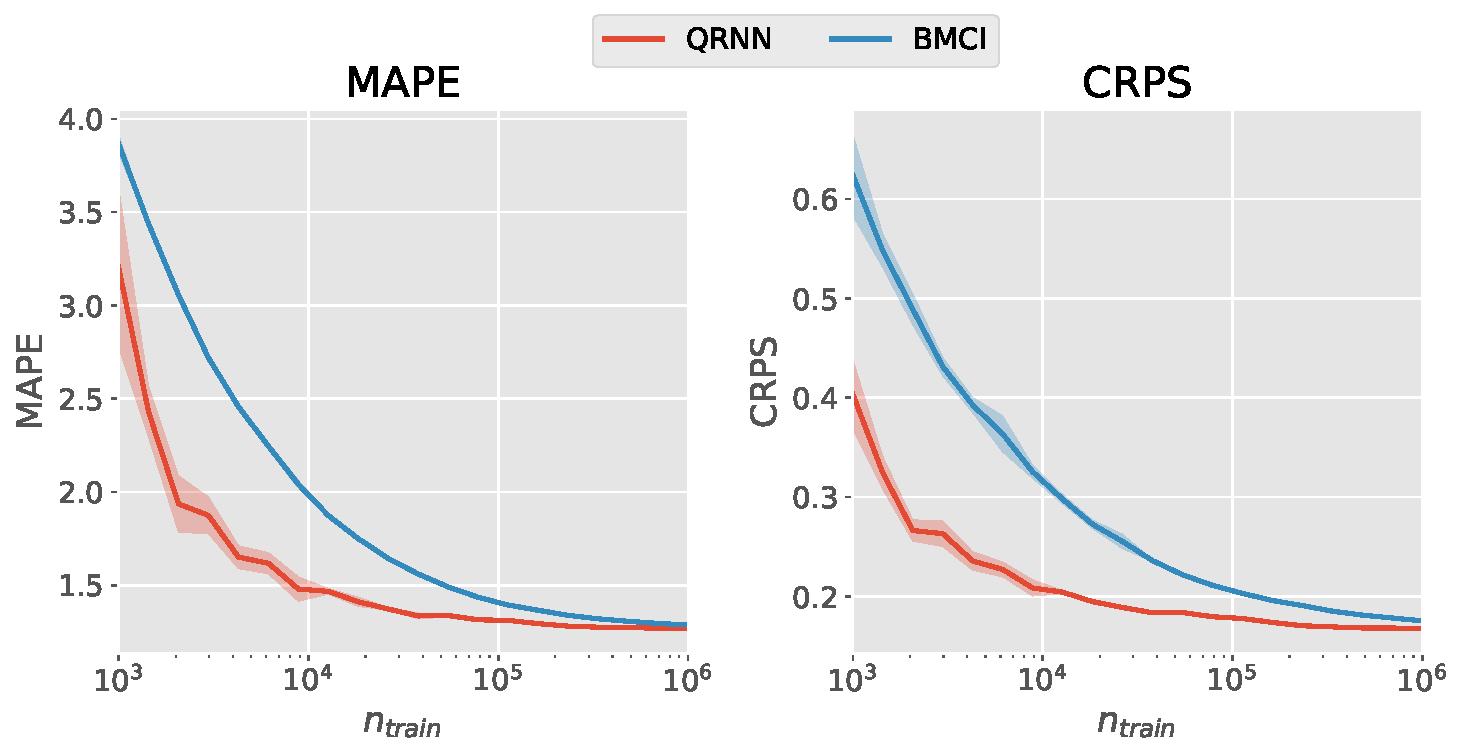
\includegraphics[width = 0.8\linewidth]{../plots/mape_crps}
    \caption{MAPE (left) and CRPS (right) achieved by BMCI (blue) and QRNN (red)
      on the test set using differently sized training subsets. For each size,
      five random subsets of the original training set were generated and used
      as training set for the QRNN and retrieval database for BMCI.}
    \label{fig:mape_crps}
  \end{figure}

Finally, also the mean of the quantile loss $\mathcal{L}_\tau$ on the test set
for $\tau = 0.1, 0.5, 0.9$ has been considered
(Figure~\ref{fig:quantile_losses}). Qualitatively, the results are similar to
the ones obtained using MAPE and CRPS. Again, the QRNN outperforms BMCI for
smaller training set sizes but the performance of the losses converge for
a training set size of $10^6$.

  \begin{figure}[hbpt!]
    \centering
    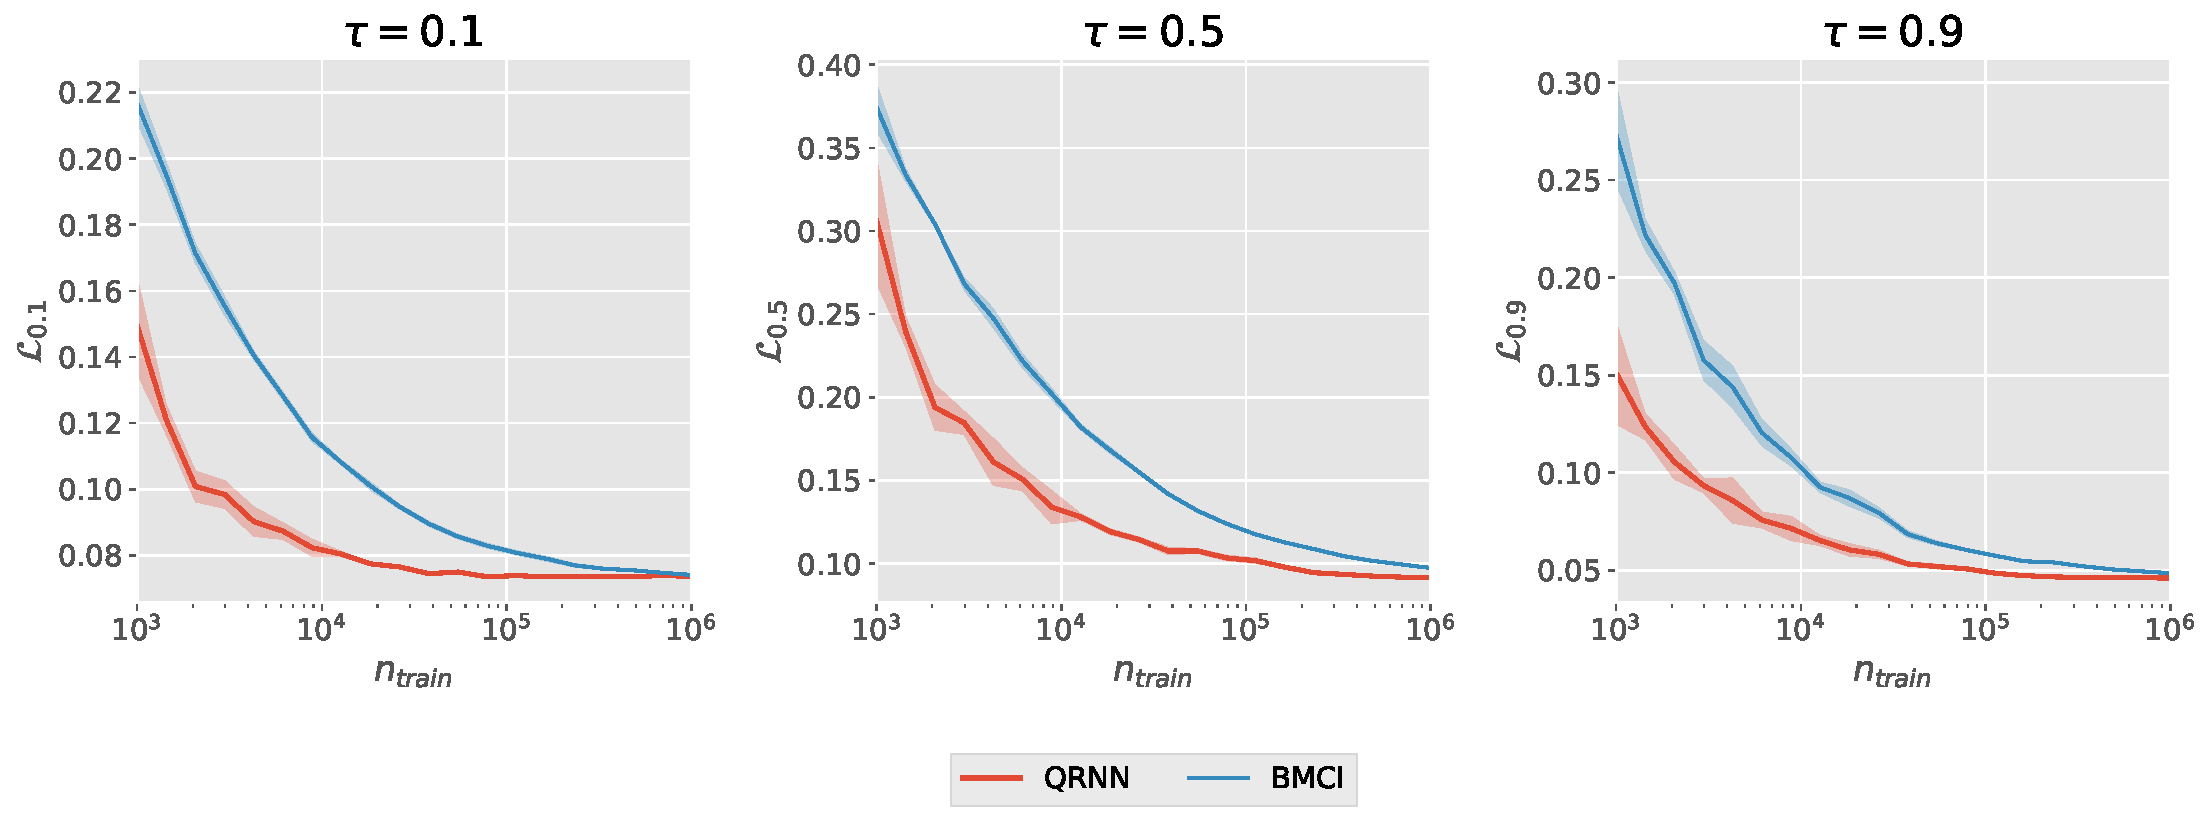
\includegraphics[width = 0.8\linewidth]{../plots/quantile_losses}
    \caption{Mean quantile loss for different training set size $n_\text{train}$ and
    $\tau = 0.1, 0.5, 0.9$.}
    \label{fig:mape_crps}
  \end{figure}

The results presented in this section indicate that while both, QRNNs and
BMCI, provide equally good predictions of the posterior distribution for the
largest training set, the neural network performs better for smaller amounts
of data. In all test cases the QRNN reaches maximum performance already for
training set size of $10^5$ which is an order of magnitude less training data
than BMCI requires to reach its performance maximum.

\section{Retrieving Cloud Top Pressure from MODIS using QRNNs}
\label{sec:ctp}

In this section QRNNs are applied to retrieve cloud top pressure from MODIS
observations. This experiment is based on the work by \cite{hakansson} who
developed a cloud top pressure retrieval algorithm (NN-CTTH) based on neural
networks. The QRNNs are compared to the NN-CTTH algorithm and it is investigated
how QRNNs can be used to estimate the retrieval uncertainty.

\subsection{Data}

For the training of the QRNNs exactly the same data as for the training of the
NN-CTTH algorithm is used. It consists of pixels of MODIS observations collocated
with CALIPSO data from which the cloud top pressure is extracted. The algorithm
uses only the $11 \unit{\mu m}$ and $12\unit{\mu m}$ channels of MODIS to make the
algorithm applicable to a broader range of sensors. In addition to the single pixel
input, structural information is provided to the neural network in the form of various
statistics computed on a $5 \times 5$ neighborhood around the pixel. Furthermore,
numerical weather prediction data is provided to the network in the form
of surface pressure, temperatures at several height levels, and predicted column
integrated water vapor.

The data used for the training of the QRNNs are the \textit{training and during-training
validation set} from the original article \citep{hakansson}. For the comparison to
NN-CTTH, the dataset for \textit{testing under development} is used.

\subsection{Training}

For the training of the QRNNs the same training scheme as described in
Section~\ref{sec:implementation} is used. The during-training validation
set is used to monitor training progress based on which the learning rate
is reduced or the training stopped.

After performing a grid search over width, depth and minibatch size, the best
performance on the validation set has been obtained for networks consisting of
four hidden layers with 64 neurons and a batch size of 128 samples.

The training was performed using adversarial training to improve the calibration
of the probabilistic predictions. A plot of the calibration of the prediction
intervals derived from a single QRNN is displayed in
Figure~\ref{fig:validation_calibration}. The data used to generate this plot is
the during-training validation set. Without adversarial training
($\delta_\text{adv} = 0$) the predictions obtained from the QRNN are overly
confident, leading to prediction intervals that underrepresent the uncertainty
in the retrieval. Adversarial training may be viewed as a way of introducing
observation uncertainty into the training data and hence larger values of
$\delta_\text{adv}$ lead to less confident predictions of uncertainty. Based on
these results, $\delta_\text{adv} = 0.05$ is chosen for the training of the
network.

These hyperparameters have been used to train a simple QRNN as well as
an ensemble of five QRNNs.

  \begin{figure}[hbpt!]
    \centering
    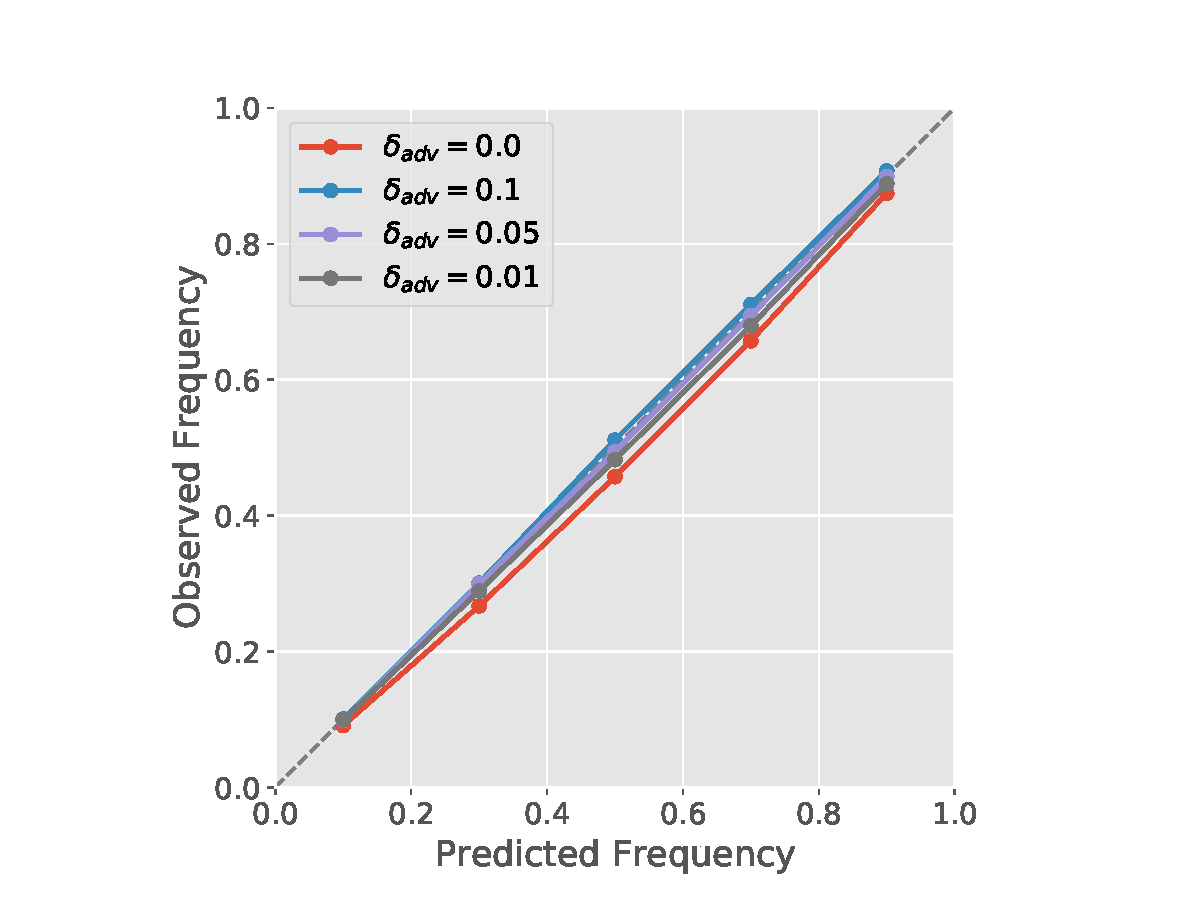
\includegraphics[width = 0.4\linewidth]{../plots/validation_calibration}
    \caption{Calibration of the QRNN prediction intervals on the validation set
      used during training. The curves display the results for no adversarial training
      ($\delta_\text{adv} = 0$) and adversarial training with perturbation
      factor $\delta_\text{adv} = 0.01, 0.05, 0.1$.}
    \label{fig:validation_calibration}
  \end{figure}


\subsection{Prediction Accuracy}


  Figure~\ref{fig:ctp_results} displays the distributions of the errors of the
  predicted cloud top pressures on the data set for testing during development.
  For the QRNNs, the prediction is taken as the median of the posterior
  distribution. Both, the simple QRNN and the ensemble of QRNNs, perform
  slightly better than the NN-CTTH algorithm for low and high clouds. For medium
  clouds, no significant difference in the performance of the methods can be
  observed. The ensemble of QRNNs seems to slightly improve upon the prediction
  accuracy of a single QRNN but the difference in accuracy is likely negligible.

  \begin{figure}[hbpt!]
    \centering
    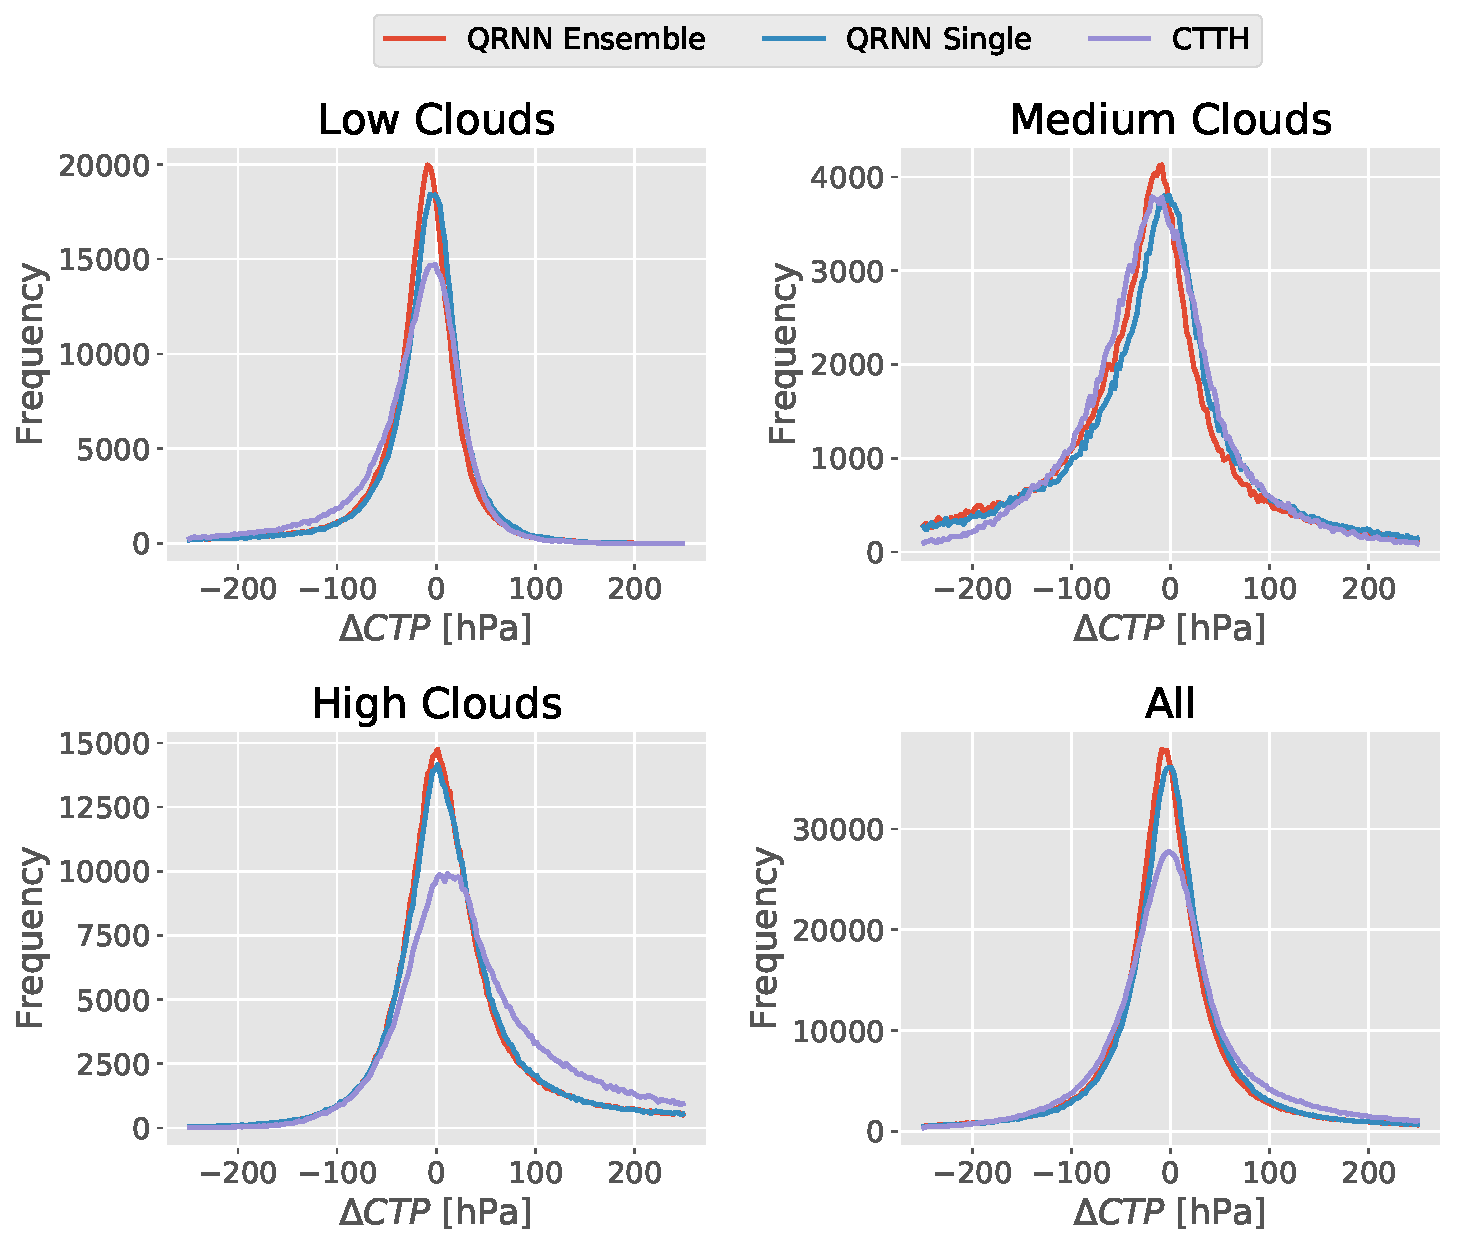
\includegraphics[width = 0.8\linewidth]{../plots/ctp_results}
    \caption{Error distributions of predicted cloud top pressure for different cloud types as well as
    the complete test set.}
    \label{fig:ctp_results}
  \end{figure}

\subsection{Uncertainty Estimation}

The NN-CTTH algorithm only retrieves cloud top pressure and does not provide
case-specific uncertainty estimates. Rather, an estimate of uncertainty is
provided in the form of the observed mean absolute error on the test set. In
order to compare these uncertainty estimates with those obtained using QRNNs,
Gaussian error distributions are fitted to the observed error based on the
observed mean absolute error (MAE) and mean squared error (MSE).

A plot of the observed test set error and the fitted Gaussian error
distributions is displayed in the left panel of Figure~\ref{fig:error_fit}. The
middle panel displays the observed error together with the predicted error
obtained from a single QRNN. The predicted error is computed as the deviation of
a randomly drawn sample of the estimated posterior distributions from the
median. These results indicate that the fitted Gaussian error distribution does
not provide a very good fit to the error that is actually observed on the
validation set. The error predicted by the QRNN reproduces the error observed on
the evaluation set fairly well. This indicates that the QRNN successfully
learned to predict retrieval uncertainties. Furthermore, the results show that
the ensemble of QRNNs actually provides a slightly worse fit to the observed
error than a single QRNN. This indicates that an ensemble of QRNNs does not
necessarily improve the calibration of the predictions.

  \begin{figure}[hbpt!]
    \centering
    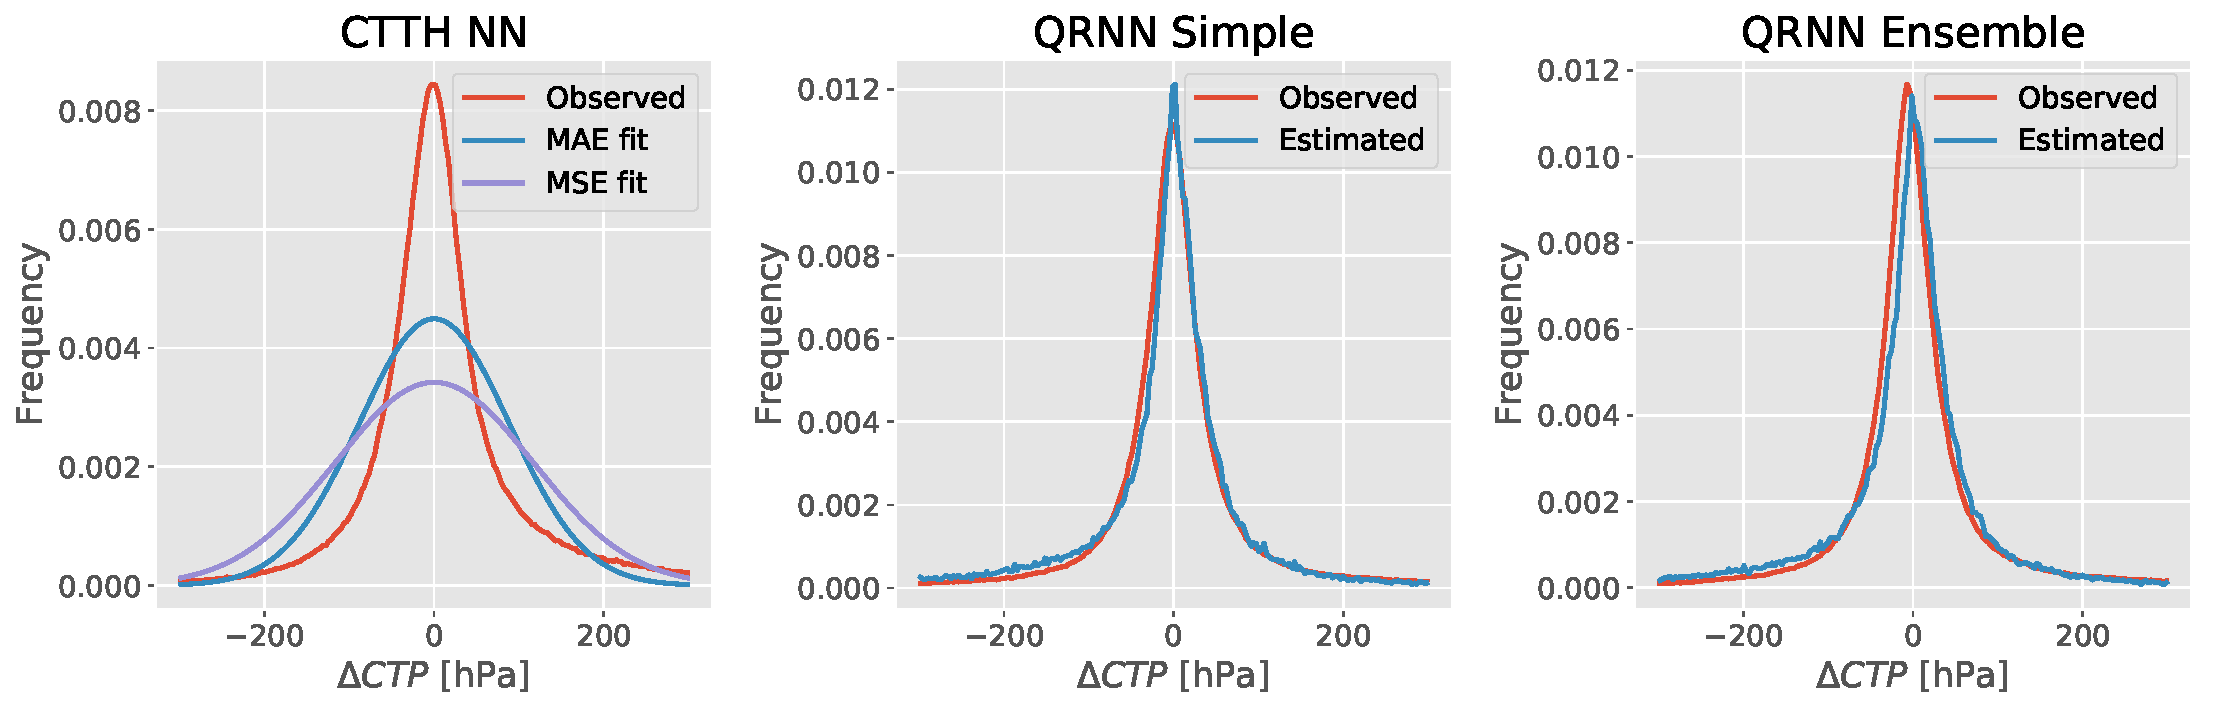
\includegraphics[width = 0.8\linewidth]{../plots/ctp_error_fit}
    \caption{Predicted and observed error distributions. The left panel
      displays the observed error for the NN-CTTH prediction as well as the
      Gaussian error distributions that have been fitted to the observed
      validation set error based on the MAE and MSE. The middle panel
      displays the observed test set error for a single QRNN as well as the
      predicted error obtained as the deviation of random sample of the
      predicted posterior from the median. The right panel displays
      the same for the ensemble of QRNNs.}
    \label{fig:error_fit}
  \end{figure}

The Gaussian error model based on the MAE fit has also been used to produce
prediction intervals for the estimated cloud pressure values obtained from the
NN-CTTH algorithm. The plot in Figure~\ref{fig:calibration} displays the
calibration of the prediction intervals obtained from the NN-CTTH predictions,
a simple QRNN as well as an ensemble of QRNNs. Also here the results show that
a single QRNN is able to provide well calibrated probabilistic predictions of
the a posteriori distribution. The ensemble of QRNNs on the other slightly
overestimates the uncertainty leading to too wide prediction intervals. The
NN-CTTH predictions are not as well calibrated and tend to provide too wide
prediction intervals for $p = 0.1, 0.3, 0.5$ but too narrow intervals for $p =
0.7$ and $p = 0.9$.

  \begin{figure}[hbpt!]
    \centering
    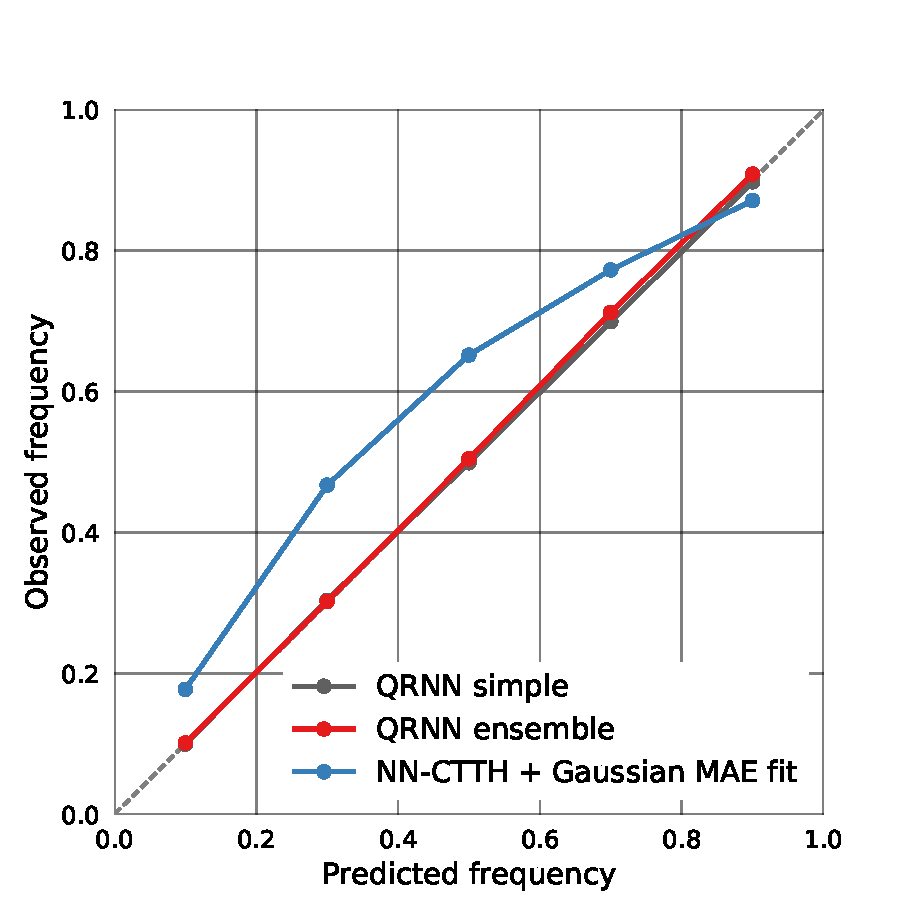
\includegraphics[width = 0.4\linewidth]{../plots/calibration_1}
    \caption{Calibration of the uncertainty estimates on the test set. Plotted in the
      figure are the predicted confidence intervals for $p = 0.1, 0.3, \ldots,
      0.9$ on the ordinate against the actually observed fraction of test values
      within these intervals on the abscissa. Displayed are the results for
      intervals obtained from a Gaussian fit to the test set error (mauve),
      as well as the prediction intervals derived from the quantiles predicted by a
      single QRNN (blue) and an ensemble of QRNNs (red).}
    \label{fig:calibration}
  \end{figure}

\subsection{Limitations}

As has been shown above, the predictions obtained from the QRNN are statistically
consistent in the sense that the prediction interval associated with confidence
$p$ indeed contains the true cloud top pressure in a fraction $p$ of the validation
cases. This however requires that the validation data itself is consistent with the
a priori distribution of the training data. What happens when this is not the case
can be seen when the calibration with respect to different cloud types is computed.
Figure~\ref{fig:calibration_cloud_type} displays the calibration plot with respect
to low, medium and high clouds. As can be seen from the plot, the predictions are
not as well calibrated as on the complete validation set.
The prediction intervals displayed for the NN-CTTH algorithm are obtained by
separate fits to the errors with respect to each cloud type. In this case the
quality of the uncertainty estimates can  even be improved for the specific
cloud types.


  \begin{figure}[hbpt!]
    \centering
    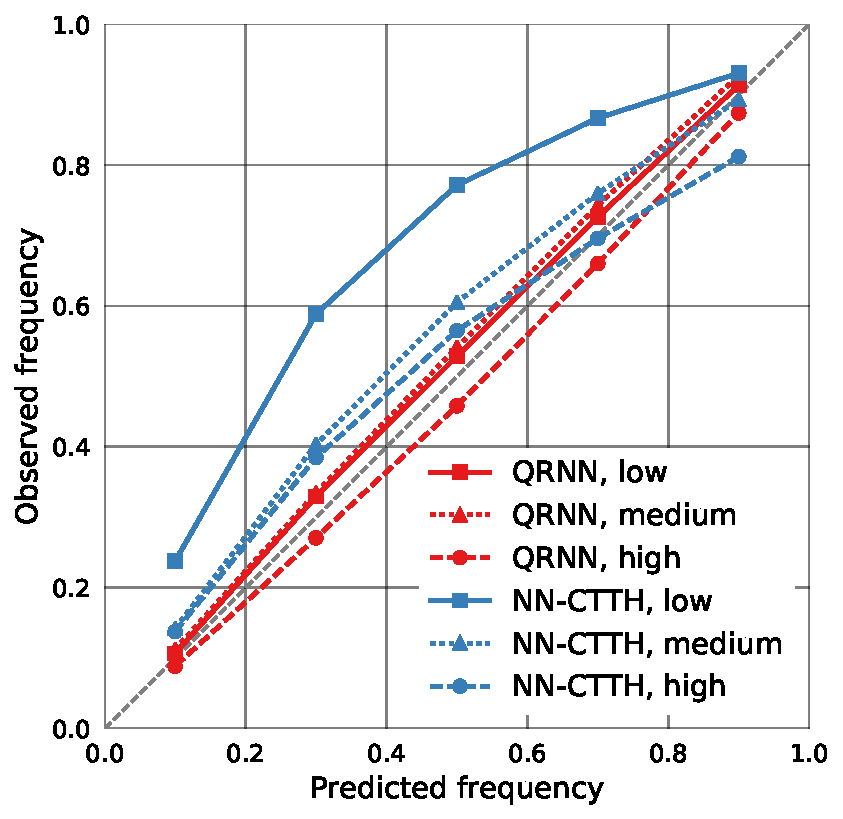
\includegraphics[width = 0.4\linewidth]{../plots/calibration_cloud_type}
    \caption{Calibration of the prediction interval obtained from NN-CTTH and QRNN
    with respect to specific cloud types.}
    \label{fig:calibration_cloud_type}
  \end{figure}


\conclusions  %% \conclusions[modified heading if necessary]

In this article, quantile regression neural networks have been proposed as a method
to estimate a posteriori distributions of Bayesian retrieval problems. Moreover,
QRNNs have been applied to two retrieval scenarios of scalar atmospheric variables.
It has been demonstrated that QRNNs are capable of providing accurate and
well-calibrated probabilistic predictions.

The synthetic retrieval case presented in Section~\ref{sec:synthetic} shows that
the conditional distribution learned by the QRNN is the same as the Bayesian
posterior distribution obtained from methods that are directly based on the
Bayesian formulation. It is interesting to note that the a priori knowledge is
implicitly represented by the distribution of the training set samples. This
Bayesian perspective not only allows for a more unified treatment of explicitly
Bayesian retrieval methods and neural network based methods, but also makes
explicit the dependence of neural network retrievals on a priori assumptions
encoded in the training data. On the synthetic dataset, the QRNN method compares
well to the BMCI method which should make it an interesting alternative to BMCI
as it allows for more flexible integration of acillary data into the retrieval.
Furthermore, QRNN retrievals can be easily parallelized and hardware optimized
implementations are available for all modern computing architectures. While the
optimization of the BMCI method has not been investigated in this work, at least
compared to a naive implementation of BMCI, QRNNs allow for up to two orders of
magnitude faster retrievals. It should be noted here, however, that these
results are of course based on the idealized assumptions of the a priori
knowledge and observation uncertainty being known exactly.

An interesting next step in this line of research would therefore be to compare
QRNNs and BMCI on a real world retrieval case.

In the second retrieval application presented in this article, QRNNs have been
used to retrieve cloud top pressure from MODIS observations. The results show
that not only are QRNNs able to improve upon state-of-the-art retrieval
accuracy but that they also can learn to predict retrieval uncertainty. The
ability of QRNNs to provide statistically consistent, case-specific uncertainty
estimates should make them a very interesting alternative to non-probabilistic
neural network retrievals. Nonetheless, also the limitations of the QRNN approach
have been demonstrated. The posterior distribution learned by the QRNN of course
depend on the validity of the a priori knowledge that is encoded in the
training data. In particular accurate uncertainty estimates can only be expected
if the retrieved observations follow the same distribution as the training data.

It is important to note that only so called in-distribution uncertainty has been
considered here. In-distribution uncertainty is the type of uncertainty that is
inherent to the retrieval and stems from limited resolution of the observation
system as well as measurement uncertainty. What has not been considered here is
out-of-distribution uncertainty which refers to uncertainty due to statistical
differences between the training data and the data to which the neural network
is applied. It has been show that ensemble methods can be used to signal
out-of-sample application of neural networks. It would therefore be interesting
to investigate if and how ensembles of QRNN can be used to detect out-of-sample
uncertainty.


%% The following commands are for the statements about the availability of data sets and/or software code corresponding to the manuscript.
%% It is strongly recommended to make use of these sections in case data sets and/or software code have been part of your research the article is based on.

\codeavailability{The implementation of the retrieval methods that were used in this article have been published as parts of the typhon \citep{typhon} software package. The source code for the calculations presented in Section~\ref{sec:sythetic} and \ref{sec:ctp} are published in the form of Jupyter notebooks in open repositories \citep{predictive_uncertainty, smhi}.}


%\dataavailability{TEXT} %% use this section when having only data sets available


%\codedataavailability{TEXT} %% use this section when having data sets and software code available





\appendix
\section{}    %% Appendix A

\subsection{}     %% Appendix A1, A2, etc.


\noappendix       %% use this to mark the end of the appendix section

%% Regarding figures and tables in appendices, the following two options are possible depending on your general handling of figures and tables in the manuscript environment:

%% Option 1: If you sorted all figures and tables into the sections of the text, please also sort the appendix figures and appendix tables into the respective appendix sections.
%% They will be correctly named automatically.

%% Option 2: If you put all figures after the reference list, please insert appendix tables and figures after the normal tables and figures.
%% To rename them correctly to A1, A2, etc., please add the following commands in front of them:

\appendixfigures  %% needs to be added in front of appendix figures

\appendixtables   %% needs to be added in front of appendix tables

  \begin{table}[ht]
  \begin{center}

    \vspace{0.5cm}
    \resizebox{\textwidth}{!}{
     \begin{tabular}{|l|ccccccc|}
     \multicolumn{8}{c}{Linear}\\
     \hline
     \input{../tables/linear.tbl}
     \end{tabular}}

    \vspace{0.5cm}
    \resizebox{\textwidth}{!}{
     \begin{tabular}{|l|ccccccc|}
     \multicolumn{8}{c}{Sigmoid}\\
     \hline
     \input{../tables/sigmoid.tbl}
     \end{tabular}}

    \vspace{0.5cm}
    \resizebox{\textwidth}{!}{
     \begin{tabular}{|l|ccccccc|}
     \multicolumn{8}{c}{tanh}\\
     \hline
     \input{../tables/tanh.tbl}
     \end{tabular}}

    \vspace{0.5cm}
    \resizebox{\textwidth}{!}{
     \begin{tabular}{|l|ccccccc|}
     \multicolumn{8}{c}{ReLU}\\
     \hline
     \input{../tables/relu.tbl}
     \end{tabular}}

    \caption{Mean quantile loss and standard deviation for different activation functions, varying numbers
             $n_h$ of hidden layers and $n_n$ of neurons per layer. Results were obtained using 10-fold
             cross validation on the training set.}

 \label{tab:model_selection}

  \end{center}
 \end{table} 

%% Please add \clearpage between each table and/or figure. Further guidelines on figures and tables can be found below.



\authorcontribution{All authors contributed to the study through discussion and feedback.
  Patrick Ericksson and Simon Pfreundschuh designed the study.
  Anke Thoss and Nina H{\aa}kansson provided the training data for the cloud top pressure
  retrieval.
  Simon Pfreundschuh implemented the code, performed the calculations and prepared the manuscript
  including figures and tables.
} %% optional section

\competinginterests{The authors declare that they have no conflict of interest.} %% this section is mandatory even if you declare that no competing interests are present

\disclaimer{TEXT} %% optional section

\begin{acknowledgements}
TEXT
\end{acknowledgements}




%% REFERENCES

%% The reference list is compiled as follows:


%% Since the Copernicus LaTeX package includes the BibTeX style file copernicus.bst,
%% authors experienced with BibTeX only have to include the following two lines:
%%
\bibliographystyle{copernicus}
\bibliography{literature.bib}
%%
%% URLs and DOIs can be entered in your BibTeX file as:
%%
%% URL = {http://www.xyz.org/~jones/idx_g.htm}
%% DOI = {10.5194/xyz}


%% LITERATURE CITATIONS
%%
%% command                        & example result
%% \citet{jones90}|               & Jones et al. (1990)
%% \citep{jones90}|               & (Jones et al., 1990)
%% \citep{jones90,jones93}|       & (Jones et al., 1990, 1993)
%% \citep[p.~32]{jones90}|        & (Jones et al., 1990, p.~32)
%% \citep[e.g.,][]{jones90}|      & (e.g., Jones et al., 1990)
%% \citep[e.g.,][p.~32]{jones90}| & (e.g., Jones et al., 1990, p.~32)
%% \citeauthor{jones90}|          & Jones et al.
%% \citeyear{jones90}|            & 1990



%% FIGURES

%% When figures and tables are placed at the end of the MS (article in one-column style), please add \clearpage
%% between bibliography and first table and/or figure as well as between each table and/or figure.


%% ONE-COLUMN FIGURES

%%f
%\begin{figure}[t]
%\includegraphics[width=8.3cm]{FILE NAME}
%\caption{TEXT}
%\end{figure}
%
%%% TWO-COLUMN FIGURES
%
%%f
%\begin{figure*}[t]
%\includegraphics[width=12cm]{FILE NAME}
%\caption{TEXT}
%\end{figure*}
%
%
%%% TABLES
%%%
%%% The different columns must be seperated with a & command and should
%%% end with \\ to identify the column brake.
%
%%% ONE-COLUMN TABLE
%
%%t
%\begin{table}[t]
%\caption{TEXT}
%\begin{tabular}{column = lcr}
%\tophline
%
%\middlehline
%
%\bottomhline
%\end{tabular}
%\belowtable{} % Table Footnotes
%\end{table}
%
%%% TWO-COLUMN TABLE
%
%%t
%\begin{table*}[t]
%\caption{TEXT}
%\begin{tabular}{column = lcr}
%\tophline
%
%\middlehline
%
%\bottomhline
%\end{tabular}
%\belowtable{} % Table Footnotes
%\end{table*}
%
%
%%% MATHEMATICAL EXPRESSIONS
%
%%% All papers typeset by Copernicus Publications follow the math typesetting regulations
%%% given by the IUPAC Green Book (IUPAC: Quantities, Units and Symbols in Physical Chemistry,
%%% 2nd Edn., Blackwell Science, available at: http://old.iupac.org/publications/books/gbook/green_book_2ed.pdf, 1993).
%%%
%%% Physical quantities/variables are typeset in italic font (t for time, T for Temperature)
%%% Indices which are not defined are typeset in italic font (x, y, z, a, b, c)
%%% Items/objects which are defined are typeset in roman font (Car A, Car B)
%%% Descriptions/specifications which are defined by itself are typeset in roman font (abs, rel, ref, tot, net, ice)
%%% Abbreviations from 2 letters are typeset in roman font (RH, LAI)
%%% Vectors are identified in bold italic font using \vec{x}
%%% Matrices are identified in bold roman font
%%% Multiplication signs are typeset using the LaTeX commands \times (for vector products, grids, and exponential notations) or \cdot
%%% The character * should not be applied as mutliplication sign
%
%
%%% EQUATIONS
%
%%% Single-row equation
%
%\begin{equation}
%
%\end{equation}
%
%%% Multiline equation
%
%\begin{align}
%& 3 + 5 = 8\\
%& 3 + 5 = 8\\
%& 3 + 5 = 8
%\end{align}
%
%
%%% MATRICES
%
%\begin{matrix}
%x & y & z\\
%x & y & z\\
%x & y & z\\
%\end{matrix}
%
%
%%% ALGORITHM
%
%\begin{algorithm}
%\caption{...}
%\label{a1}
%\begin{algorithmic}
%...
%\end{algorithmic}
%\end{algorithm}
%
%
%%% CHEMICAL FORMULAS AND REACTIONS
%
%%% For formulas embedded in the text, please use \chem{}
%
%%% The reaction environment creates labels including the letter R, i.e. (R1), (R2), etc.
%
%\begin{reaction}
%%% \rightarrow should be used for normal (one-way) chemical reactions
%%% \rightleftharpoons should be used for equilibria
%%% \leftrightarrow should be used for resonance structures
%\end{reaction}
%
%
%%% PHYSICAL UNITS
%%%
%%% Please use \unit{} and apply the exponential notation


\end{document}
